\documentclass{article}

\usepackage{tikz}


\begin{document}

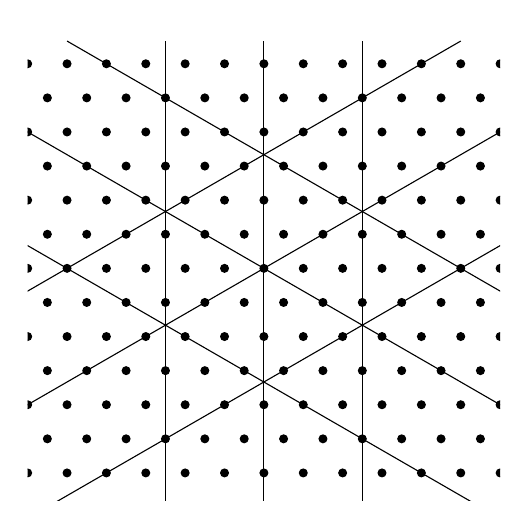
\begin{tikzpicture}[scale=.5]
 
\clip (-9, -3)--(3,-3)--(3,9)--(-9,9)--cycle;

\draw (-.5, 10*1.7320508/2)--(-.5, -5*1.7320508);
\draw (-3, 10*1.7320508/2)--(-3, -5*1.7320508);
\draw (-5.5, 10*1.7320508/2)--(-5.5, -5*1.7320508);

\draw (-15-3, 5*1.7320508)--(15-3, -5*1.7320508);
\draw (-15-3+5, 5*1.7320508)--(15-3+5, -5*1.7320508);
\draw (-15-3+10, 5*1.7320508)--(15-3+10, -5*1.7320508);


\draw (-15-3, -5*1.7320508)--(15-3, 5*1.7320508);
\draw (-15-3-5, -5*1.7320508)--(15-3-5, 5*1.7320508);
\draw (-15-3-10, -5*1.7320508)--(15-3-10, 5*1.7320508);

\begin{scope}[yshift=-.33333333333*1.7320508cm]
\foreach \x in {-10,...,10}{% Two indices running over each
    \foreach \y in {-10,...,10}{% node on the grid we have drawn
        \node[draw,circle,inner sep=1pt,fill] at (\x-\y/2,1.7320508*\y/2) {};}}
\end{scope}


\end{tikzpicture}


\end{document}